%!TEX root = ../Electrodynamics.tex
<<<<<<< HEAD

\subsection{}
=======
\subsection{Телеграфные уравнения для идеальной линии. Погонные параметры линии. Волновое уравнения, общий вид его решения. Понятие волнового сопротивления линии в терминах тока и напряжения}

\begin{figure}[h!]
	\centering
	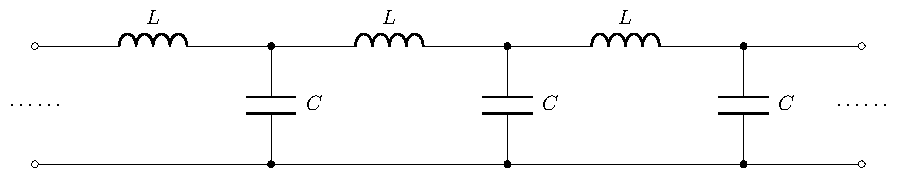
\includegraphics[width = 0.4\linewidth]{img/task7_ris1.pdf}
\end{figure}

Теория в первую очередь применяется для $TEM$-волн. В описании  применяют цепочки.
$\lambda \gg l$, $l$-- размер одного звена цепи.  $C$-- погонная емкость, $L$-- погонная индуктивность.

Рассмотрим двупроводную линию. $Q$-- заряд на единицу длины этой линии. Рассмотрим сечение этой двупроводной линии $z=\const$. Напряжение между двумя проводами в этом сечении запишется как:
\begin{equation}
	V(z)=\int\limits_{(1)}^{(2)} E_l \dd{l},
\end{equation}
этот интеграл в сечении $z=\const$ \textbf{не будет} зависеть от формы контура, поскольку структура поля $\vec E$ в $TEM$-волне электростатична.

\begin{gather}
	\vec E = \vec E_\perp\\
	\vec E_\perp= - \grad_\perp \phi\\
	\Delta_\perp \phi = 0 + \text{гр.усл.}
\end{gather}
А это и означает, что поле $\vec E$ потенциально в перпендикулярном направлении. При этом 
\begin{equation}
	\Rot \vec E = \Rot\qty[\grad_\perp \phi(\vec r_\perp) e^{-ihz}] \neq 0
\end{equation}
Уравнения, связывающие ток $I$ и напряжение $V$ называются телеграфными. Они получаются из законов Кирхгофа.

Приращение заряда $\Delta q= Q \Delta z$ на участке $\Delta z$ за время $\Delta t$ равно:

\begin{gather}
	\Delta(\Delta q) = \Delta q(t + \Delta t) - \Delta q(t)
\end{gather}
С другой стороны, изменение заряда есть разность подтекающих и оттекающих токов:
\begin{equation}
	\pdv{t} (\Delta q )= I(z)-I(z+ \Delta z)= \pdv{t} (Q \Delta z)
\end{equation}
Осталось только выполнить предельный переход.  Из закона сохранения заряда следует \textbf{первое телеграфное уравнение}:
\begin{equation}
	\pdv{Q}{t}= - \pdv{I}{z}
\end{equation}

Второе уравнение получим из закона электромагнитной индукции
\begin{equation}
	\oint E_l \dd{l}= \frac{1}{c} \pdv{t} \underbrace{\iint  \vec B \dd{\vec S}}_{\Delta \psi} = V(z+ \Delta z) - V(z)
\end{equation}
По определению индуктивности:
\begin{equation}
	\Delta \psi = \frac{\Delta L}{c} I = \frac{L \Delta z}{c} I
\end{equation}

Получаем \textbf{второе телеграфное уравнение}
\begin{equation}
	\pdv{V}{z} = - \frac{1}{c^2} L \pdv{I}{t}
\end{equation}

>>>>>>> origin/Kirill

